\documentclass[12pt]{article}

\usepackage{graphicx}
\usepackage{hyperref}
\usepackage{listings}

\setlength{\textheight}{8.5in}
\setlength{\headheight}{.25in}
\setlength{\headsep}{.25in}
\setlength{\topmargin}{0in}
\setlength{\textwidth}{6.5in}
\setlength{\oddsidemargin}{0in}
\setlength{\evensidemargin}{0in}

\title{PartyUp Internals}
\author{David Gilhooley, Lance Goodridge, Blake Lawson, and Graham Turk}

\begin{document}

\pagestyle{plain}

\maketitle

\section{Overview}

PartyUp is an iOS app written in Swift.
The app's back end is hosted on an Amazon Web Services (AWS)
EC2 instance running Ubuntu.
The back end is built using the Django web framework and uses
a MySQL database.
PartyUp uses Git for version control and the code for the project is 
hosted on \href{https://github.com/}{GitHub}.
The iOS code and back end code can be found at 
\url{https://github.com/BDGL-Hacks/iOS-333} and
\url{https://github.com/BDGL-Hacks/backend-333} respectively.


\section{Implementation: Front End}

Gonna put more sick graphics here

\section{Implementation: Back End}

At a high level, there are a few major components to the back end:
an AWS EC2 instance, an AWS S3 bucket, Pusher, and the Apple Push Notification Service (APNS).
Figure~\ref{fig:stack} contains a graphical representation of the system.
All of the functions in the PartyUp API are documented on GitHub
in the \href{https://github.com/BDGL-Hacks/backend-333/wiki}{project wiki},
and all of the Python code is written according to the PEP-8 Python standard.

\begin{figure}[h]
    \centering
    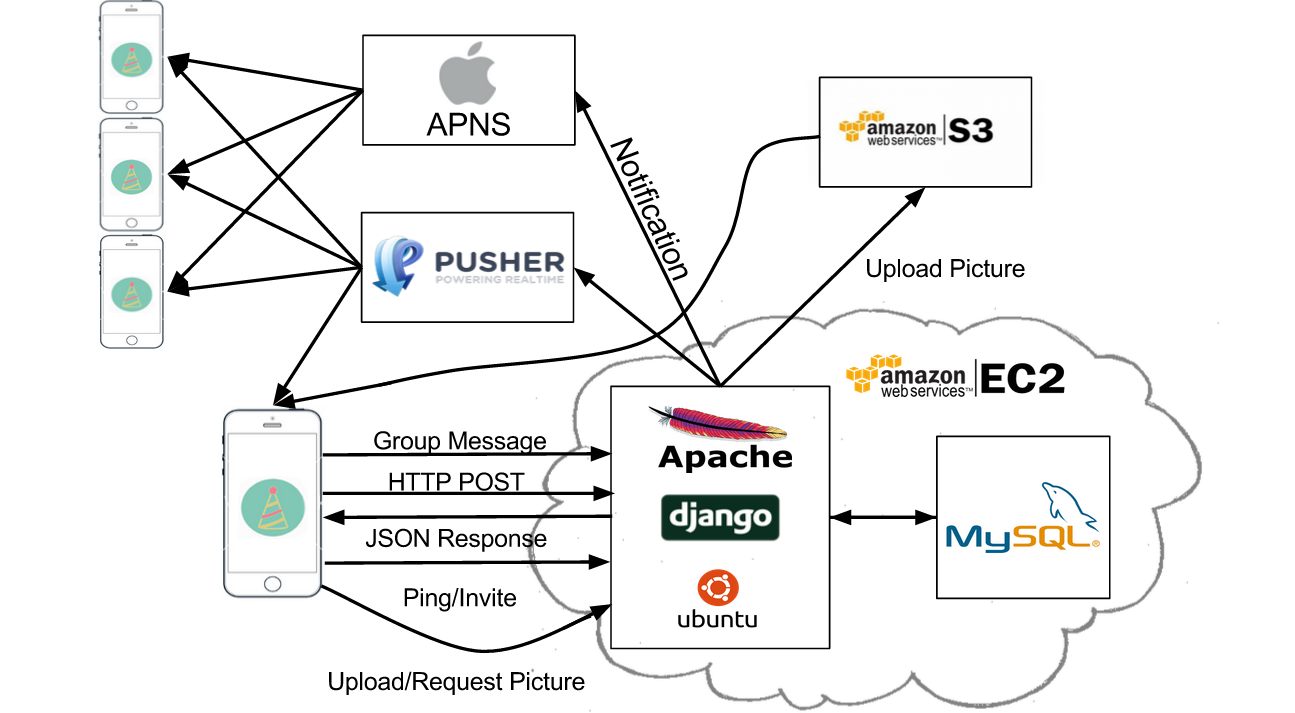
\includegraphics[scale=0.4]{Stack.png}
    \caption{
        A simplified map of the PartyUp back end. 
    }
    \label{fig:stack}
\end{figure}


In this section, we will give an overview each of major components in this system
in the context of the code found in the
\href{https://github.com/BDGL-Hacks/backend-333}{backend-333 directory}.
At the top level, there are a few files and sub-directories.

\texttt{curl.sh} is a short bash script that is basically a wrapper for 
\texttt{cURL} that makes it a little easier to test the back end API.

\texttt{requirements.txt} is a list of Python packages that are needed to
run all of the Python programs within the directory.
All of the packages can be installed using \texttt{pip}, the recommended
Python package manager.
The command
\begin{lstlisting}
    pip install -r requirements.txt
\end{lstlisting}
will install all of the packages at once.

The two directories, \texttt{testdata} and \texttt{partyup} will be covered
in greater detail below.

\subsection{testdata}

This directory contains a Python script, \texttt{filldatabase.py},
which can be used to fill the PartyUp database with test data
found in the accompanying files, \texttt{users.txt} and \texttt{events.txt}.
The files themselves are well documented and contain information about
how to run the script.

\subsection{partyup}

This directory contains the Django project, and thus,
it contains most of the code for the back end.
For the most part, the files are structured in the way you would
expect in your typical Django project
(see \url{https://docs.djangoproject.com/en/1.7/} for an introduction to Django),
although there are a few exceptions.

\end{document}